\documentclass[12pt,a4paper]{article}

\usepackage[T1]{fontenc}
\usepackage[utf8]{inputenc}
\usepackage[margin=2.5cm]{geometry}
\usepackage{lmodern}
\usepackage{microtype}
\usepackage{parskip}
\usepackage{titlesec}
\usepackage{booktabs}
\usepackage{xcolor}
\usepackage{hyperref}
\usepackage{listings}
\usepackage{tikz}
\usetikzlibrary{shapes,arrows,positioning,fit,backgrounds,calc}

% ── Colours ───────────────────────────────────────────────────────────────────
\definecolor{mpblue}{HTML}{1A73E8}
\definecolor{mpgreen}{HTML}{34A853}
\definecolor{mporange}{HTML}{EA8600}
\definecolor{mppurple}{HTML}{9C27B0}
\definecolor{mpgray}{HTML}{5F6368}
\definecolor{mpred}{HTML}{EA4335}
\definecolor{codebg}{HTML}{F8F9FA}
\definecolor{codeframe}{HTML}{DADCE0}
\definecolor{skincolor}{HTML}{FDBCB4}

\hypersetup{colorlinks=true, linkcolor=mpblue, urlcolor=mpblue,
    pdftitle={MediaPipe Tutorial 02 -- Face Detection and Mesh}}

\lstdefinestyle{pythonstyle}{
    language=Python, backgroundcolor=\color{codebg},
    frame=single, framerule=0.8pt, rulecolor=\color{codeframe},
    basicstyle=\ttfamily\small,
    keywordstyle=\color{mpblue}\bfseries,
    stringstyle=\color{mpgreen},
    commentstyle=\color{mpgray}\itshape,
    numberstyle=\tiny\color{mpgray},
    numbers=left, numbersep=8pt,
    breaklines=true, showstringspaces=false, tabsize=4,
}
\lstset{style=pythonstyle}

\titleformat{\section}{\large\bfseries\color{mpblue}}{}{0em}{}[\titlerule]
\titleformat{\subsection}{\normalsize\bfseries\color{mpgray}}{}{0em}{}

% ── TikZ styles ───────────────────────────────────────────────────────────────
\tikzset{
    facenode/.style={circle, draw=#1, fill=#1!20,
        minimum size=6pt, inner sep=0pt},
    regionlabel/.style={font=\tiny, color=#1, align=center},
    connline/.style={draw=#1, line width=0.8pt},
}

% ─────────────────────────────────────────────────────────────────────────────
\begin{document}

\title{\textbf{\textcolor{mpblue}{MediaPipe Tutorial 02}}\\[0.4em]
    \large Face Detection \& Face Mesh: BlazeFace, 478 Landmarks,\\
    Distance Estimation, and Multi-Face Tracking}
\author{MediaPipe Tutorials Series}
\date{\today}
\maketitle
\tableofcontents
\newpage

% ─────────────────────────────────────────────────────────────────────────────
\section{Introduction}

MediaPipe provides two complementary face models: \textbf{BlazeFace} for fast face
detection and \textbf{Face Mesh} for dense 478-landmark geometry. This tutorial covers both,
plus distance estimation and multi-face ID tracking.

% ─────────────────────────────────────────────────────────────────────────────
\section{Annotated Face Landmark Diagram}

The diagram below shows the major landmark \emph{regions} on a schematic face,
using coloured nodes and labelled groups. Actual indices are noted for key points.

\bigskip

\begin{center}
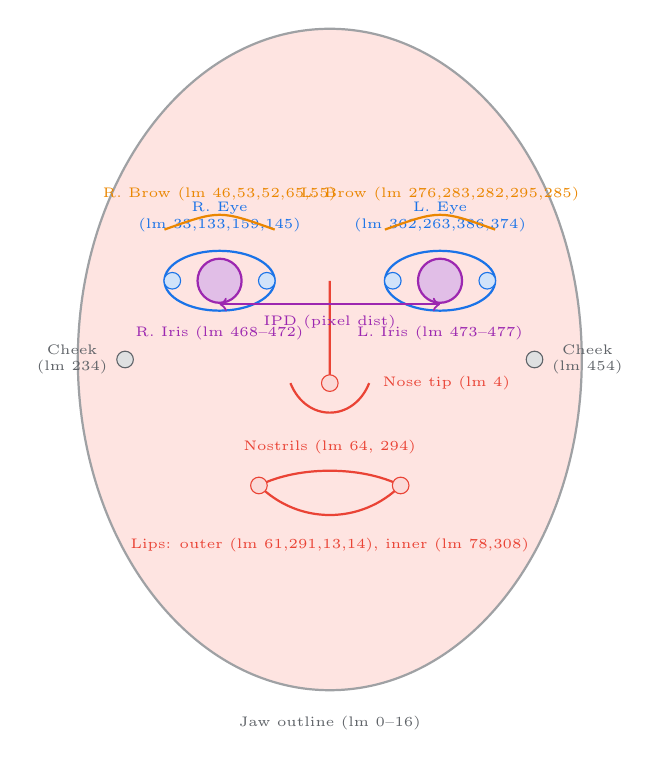
\begin{tikzpicture}[scale=1.0]

    % ── Face oval ──────────────────────────────────────────────────────────
    \draw[thick, color=mpgray!60, fill=skincolor!40]
        (0,0) ellipse (3.2cm and 4.2cm);

    % ── Jaw label ──────────────────────────────────────────────────────────
    \node[regionlabel=mpgray, below] at (0,-4.4) {Jaw outline (lm 0--16)};

    % ── Right eye region ───────────────────────────────────────────────────
    \draw[connline=mpblue] (-1.4,1.0) ellipse (0.7cm and 0.38cm);
    \node[facenode=mpblue] at (-2.0,1.0) {};   % outer corner
    \node[facenode=mpblue] at (-0.8,1.0) {};   % inner corner
    \node[regionlabel=mpblue, above] at (-1.4,1.5)
        {R. Eye\\(lm 33,133,159,145)};

    % ── Left eye region ────────────────────────────────────────────────────
    \draw[connline=mpblue] (1.4,1.0) ellipse (0.7cm and 0.38cm);
    \node[facenode=mpblue] at (0.8,1.0) {};
    \node[facenode=mpblue] at (2.0,1.0) {};
    \node[regionlabel=mpblue, above] at (1.4,1.5)
        {L. Eye\\(lm 362,263,386,374)};

    % ── Right iris ─────────────────────────────────────────────────────────
    \draw[connline=mppurple, fill=mppurple!30]
        (-1.4,1.0) circle (0.28cm);
    \node[regionlabel=mppurple, below] at (-1.4,0.55)
        {R. Iris (lm 468--472)};

    % ── Left iris ──────────────────────────────────────────────────────────
    \draw[connline=mppurple, fill=mppurple!30]
        (1.4,1.0) circle (0.28cm);
    \node[regionlabel=mppurple, below] at (1.4,0.55)
        {L. Iris (lm 473--477)};

    % ── Eyebrows ───────────────────────────────────────────────────────────
    \draw[connline=mporange, thick]
        (-2.1,1.65) .. controls (-1.4,1.9) .. (-0.7,1.65);
    \node[regionlabel=mporange] at (-1.4,2.1)
        {R. Brow (lm 46,53,52,65,55)};

    \draw[connline=mporange, thick]
        (0.7,1.65) .. controls (1.4,1.9) .. (2.1,1.65);
    \node[regionlabel=mporange] at (1.4,2.1)
        {L. Brow (lm 276,283,282,295,285)};

    % ── Nose ───────────────────────────────────────────────────────────────
    \draw[connline=mpred]
        (0,1.0) -- (0,-0.3)
        (-0.5,-0.3) .. controls (-0.3,-0.8) and (0.3,-0.8) .. (0.5,-0.3);
    \node[facenode=mpred] at (0,-0.3) {};
    \node[regionlabel=mpred, right] at (0.55,-0.3)
        {Nose tip (lm 4)};
    \node[regionlabel=mpred, below] at (0,-0.9)
        {Nostrils (lm 64, 294)};

    % ── Lips ───────────────────────────────────────────────────────────────
    % Upper lip
    \draw[connline=mpred, thick]
        (-0.9,-1.6) .. controls (-0.4,-1.35) and (0.4,-1.35) .. (0.9,-1.6);
    % Lower lip
    \draw[connline=mpred, thick]
        (-0.9,-1.6) .. controls (-0.4,-2.1) and (0.4,-2.1) .. (0.9,-1.6);
    \node[facenode=mpred] at (-0.9,-1.6) {};
    \node[facenode=mpred] at ( 0.9,-1.6) {};
    \node[regionlabel=mpred, below] at (0,-2.15)
        {Lips: outer (lm 61,291,13,14), inner (lm 78,308)};

    % ── Cheekbones ─────────────────────────────────────────────────────────
    \node[facenode=mpgray] at (-2.6,0.0) {};
    \node[regionlabel=mpgray, left] at (-2.7,0.0) {Cheek\\(lm 234)};
    \node[facenode=mpgray] at ( 2.6,0.0) {};
    \node[regionlabel=mpgray, right] at (2.7,0.0) {Cheek\\(lm 454)};

    % ── IPD annotation ─────────────────────────────────────────────────────
    \draw[<->, thick, color=mppurple]
        (-1.4,0.7) -- (1.4,0.7)
        node[midway, below, font=\tiny\color{mppurple}] {IPD (pixel dist)};

\end{tikzpicture}
\end{center}

\bigskip

\textbf{Note:} Indices shown are representative; the full 478-landmark map is available
at \href{https://github.com/google/mediapipe/blob/master/mediapipe/modules/face_geometry/data/canonical_face_model_uv_visualization.png}{MediaPipe GitHub}.

% ─────────────────────────────────────────────────────────────────────────────
\section{BlazeFace: Face Detection API}

\begin{lstlisting}[caption={Minimal face detection}]
import cv2, mediapipe as mp
mp_fd = mp.solutions.face_detection
mp_draw = mp.solutions.drawing_utils

cap = cv2.VideoCapture(0)
with mp_fd.FaceDetection(model_selection=0,
                         min_detection_confidence=0.5) as fd:
    while cap.isOpened():
        ret, frame = cap.read()
        if not ret: break
        rgb = cv2.cvtColor(frame, cv2.COLOR_BGR2RGB)
        results = fd.process(rgb)
        if results.detections:
            for det in results.detections:
                mp_draw.draw_detection(frame, det)
        cv2.imshow("BlazeFace", frame)
        if cv2.waitKey(1) & 0xFF == ord('q'): break
cap.release(); cv2.destroyAllWindows()
\end{lstlisting}

% ─────────────────────────────────────────────────────────────────────────────
\section{Face Mesh: 478 Landmarks}

\begin{lstlisting}[caption={Face Mesh webcam demo}]
import cv2, mediapipe as mp, time
mp_fm = mp.solutions.face_mesh
mp_dr = mp.solutions.drawing_utils

cap = cv2.VideoCapture(0)
with mp_fm.FaceMesh(static_image_mode=False, max_num_faces=4,
                    refine_landmarks=True,
                    min_detection_confidence=0.5,
                    min_tracking_confidence=0.5) as fm:
    while cap.isOpened():
        ret, frame = cap.read()
        if not ret: break
        rgb = cv2.cvtColor(frame, cv2.COLOR_BGR2RGB)
        rgb.flags.writeable = False
        res = fm.process(rgb)
        rgb.flags.writeable = True
        frame = cv2.cvtColor(rgb, cv2.COLOR_RGB2BGR)
        if res.multi_face_landmarks:
            for lms in res.multi_face_landmarks:
                mp_dr.draw_landmarks(frame, lms,
                    mp_fm.FACEMESH_TESSELATION)
        cv2.imshow("Face Mesh", frame)
        if cv2.waitKey(1) & 0xFF == ord('q'): break
cap.release(); cv2.destroyAllWindows()
\end{lstlisting}

% ─────────────────────────────────────────────────────────────────────────────
\section{Face Distance Estimation via IPD}

Given the inter-pupillary distance (IPD) in pixels and known physical IPD ($\approx 63$~mm):

\[
    d = \frac{f \cdot \text{IPD}_{\text{real}}}{\text{IPD}_{\text{px}}}
\]

where $f$ is the camera focal length in pixels (approximated as $0.7 \times w$).

\begin{lstlisting}[caption={IPD-based distance estimator}]
LEFT_IRIS_IDX, RIGHT_IRIS_IDX = 468, 473
REAL_IPD_MM = 63.0

def estimate_distance(landmarks, w, h, focal_px):
    import numpy as np
    def get(idx):
        lm = landmarks.landmark[idx]
        return int(lm.x*w), int(lm.y*h)
    lx, ly = get(LEFT_IRIS_IDX)
    rx, ry = get(RIGHT_IRIS_IDX)
    ipd_px = np.hypot(lx-rx, ly-ry)
    return (focal_px * REAL_IPD_MM) / (ipd_px + 1e-9)
\end{lstlisting}

% ─────────────────────────────────────────────────────────────────────────────
\section{Performance Tips}

\begin{itemize}
    \item Use \texttt{cap.set(cv2.CAP\_PROP\_FRAME\_WIDTH, 640)} for lower latency.
    \item Set \texttt{max\_num\_faces} to the minimum required.
    \item Disable \texttt{refine\_landmarks} when iris data is unnecessary.
    \item Use \texttt{static\_image\_mode=False} for video streams.
\end{itemize}

% ─────────────────────────────────────────────────────────────────────────────
\section{Next Steps}

Proceed to Tutorial~03 to work with the 21-keypoint Hand Landmark model and build gesture
recognition applications.

\end{document}
